\documentclass[11pt]{article}
\usepackage{algorithm2e}
\usepackage[italian]{babel}
\usepackage[document]{ragged2e}
\usepackage{amsfonts, amssymb, amsmath}
\usepackage{cancel}
\usepackage{float}
\usepackage{mathtools}
\usepackage[margin=3cm]{geometry}

\tolerance=1
\emergencystretch=\maxdimen
\hyphenpenalty=10000
\hbadness=10000

\begin{document}
\graphicspath{ {./img/} }
\begin{titlepage}
    \begin{center}
        \vspace*{1.5cm}
            
        \Huge
        \textbf{IMAGING}
            
        \vspace{0.5cm}
        \LARGE
        Relazione
            
        \vspace{1.5cm}
          
        \begin{minipage}[t]{0.47\textwidth}
        \begin{center}
        	{\large{\bf Cheikh Ibrahim $\cdot$ Zaid}}\\
			{\large Matricola: \texttt{0000974909}}
        \end{center}

		\end{minipage}
		\hfill
		\begin{minipage}[t]{0.47\textwidth}\raggedleft
		\begin{center}
        	{\large{\bf Xia $\cdot$ Tian Cheng}}\\
			{\large Matricola: \texttt{0000975129}}
        \end{center}
		\end{minipage}  
            
        \vspace{6cm}
            
        Anno accademico\\
        $2021 - 2022$
            
        \vspace{0.8cm}
            
            
        \Large
        Corso di Calcolo Numerico\\
        Alma Mater Studiorum $\cdot$ Università di Bologna\\
            
    \end{center}
\end{titlepage}
\pagebreak

\section*{Introduzione}
Il progetto consiste nel ricostruire un'immagine a partire da una sua istanza alterata da uno sfocamento noto e un rumore casuale.\\
Si tratta di un problema solitamente affrontato elaborando immagini provenienti da un dispositivo di acquisizione che nel suo processo di cattura deve digitalizzare un segnale analogico. 
Per risolvere tali problemi sono note diverse formulazioni. Quelle impiegate per questo progetto sono:
\begin{itemize}
    \setlength\itemsep{0.05cm}
    \item Minimi quadrati
    \item Minimi quadrati con regolarizzazione di Tikhonov
    \item Minimi quadrati con regolarizzazione tramite variazione totale
\end{itemize}
È noto che risolvere il problema di deblur come minimi quadrati in modo diretto è mal condizionato e per questo si introducono tecniche di regolarizzazione.\\
Per misurare la qualità dei risultati verranno impiegate due metriche:
\begin{itemize}
    \setlength\itemsep{0.05cm}
    \item Mean Squared Error (MSE) \textbf{[AGGIUNGERE DESCRIZIONE]}
    \item Peak Signal-to-Noise Ratio (PSNR) \textbf{[AGGIUNGERE DESCRIZIONE]}
\end{itemize}

\section*{Esecuzione preliminare}
Per avere una visione sul comportamento delle varie formulazioni, è stata eseguita una prima sperimentazione sull'immagine in Figura \ref{fig:originale1}
\begin{figure}[H]
    \centering
    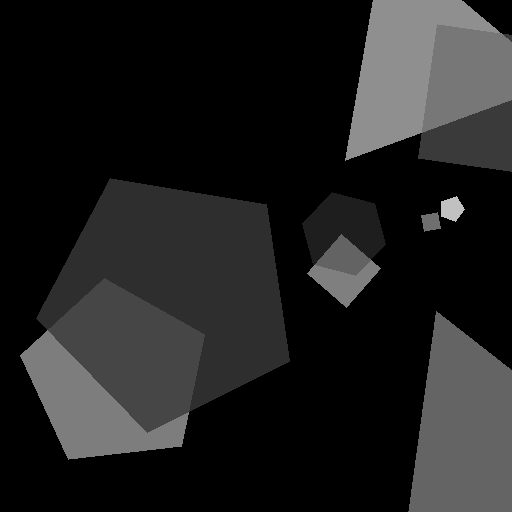
\includegraphics[width=4cm]{originale1.png}
    \caption{Immagine di test}
    \label{fig:originale1}
\end{figure}

\subsection*{Valutazione algoritmi al variare di $\lambda$}
Per valutare il risultato dei vari metodi, è necessario prima determinare il valore $\lambda$ del termine di regolarizzazione per gli algoritmi che lo prevedono.
\subsubsection*{Tikhonov}
Il seguente grafico mostra il valore del PSNR al variare di $\lambda \in [0.01, 2]$ con passo 50:
\begin{figure}[H]
    \centering
    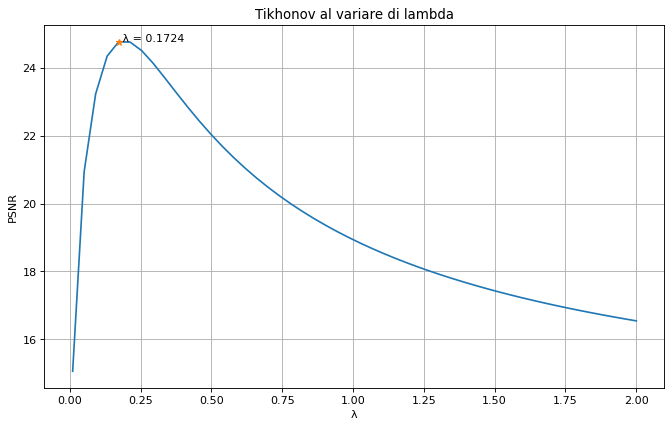
\includegraphics[width=10cm]{tikhonov_lambda1.png}
    \caption{$\lambda \simeq 0.1724$ e $\texttt{PSNR} \simeq 24.74838$}
    \label{fig:tikhonov_lambda1}
\end{figure}
Più nel dettaglio, focalizzando l'attenzione sull'intorno del punto trovato al passo precedente, il risultato con $\lambda \in [0.15, 0.3]$ è:
\begin{figure}[H]
    \centering
    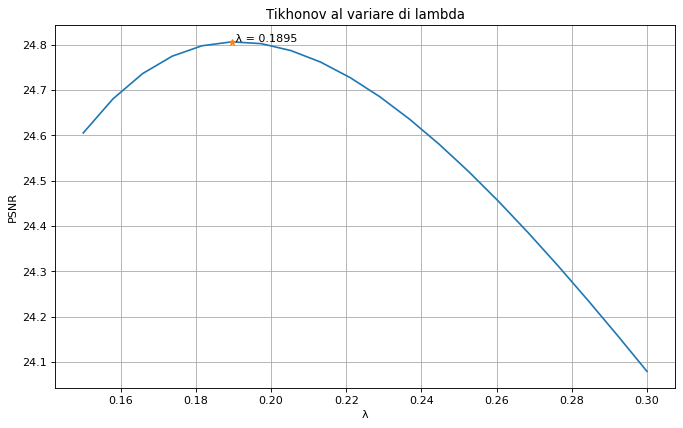
\includegraphics[width=10cm]{tikhonov_lambda2.png}
    \caption{$\lambda \simeq 0.1895$ e $\texttt{PSNR} \simeq 24.7845$}
    \label{fig:tikhonov_lambda2}
\end{figure}

\subsubsection*{Variazione totale}
Analogamente, il seguente grafico mostra il la variazione del PSNR per $\lambda \in [0.01, 2]$ con passo 50:
\begin{figure}[H]
    \centering
    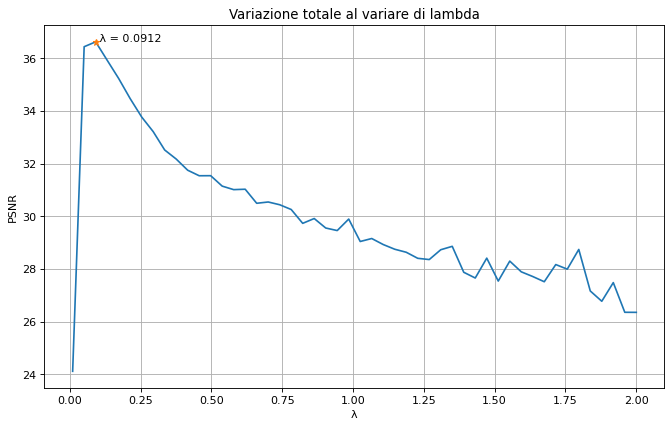
\includegraphics[width=10cm]{tv_lambda1.png}
    \caption{$\lambda \simeq 0.0912$ e $\texttt{PSNR} \simeq 36.7470$}
    \label{fig:tv_lambda1}
\end{figure}
Nell'intorno del punto trovato precedentemente, il risultato con $\lambda \in [0.08, 0.11]$ è:
\begin{figure}[H]
    \centering
    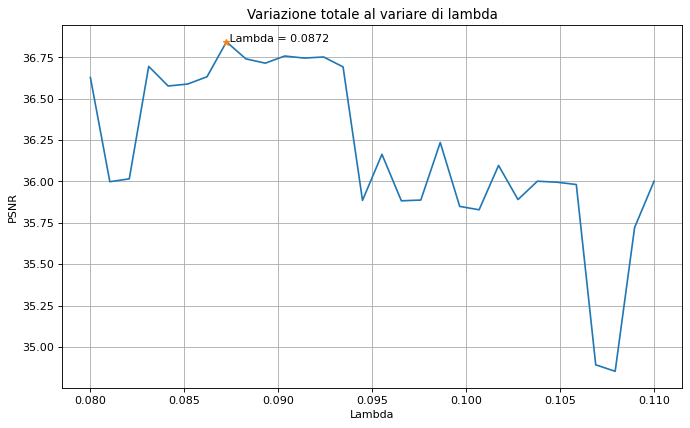
\includegraphics[width=10cm]{tv_lambda2.png}
    \caption{$\lambda \simeq 0.0872$ e $\texttt{PSNR} \simeq 36.8429$}
    \label{fig:tv_lambda2}
\end{figure}

Per avere una visione sul comportamento delle varie formulazioni, è stata eseguita una prima sperimentazione i cui risultati sono osservabili in Figura \ref{fig:deblur1}.\\
\begin{figure}[H]
    \centering
    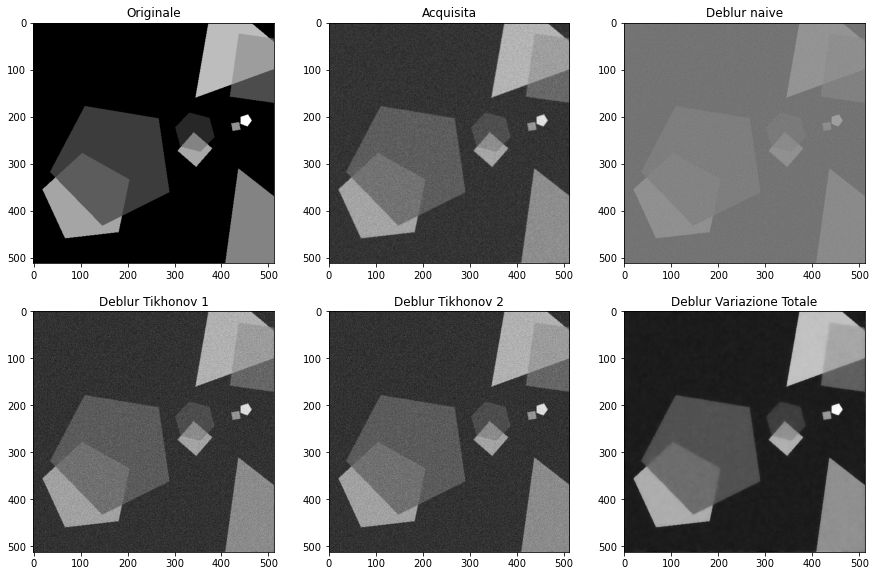
\includegraphics[width=15cm]{deblur1.png}
    \caption{Risultato sulle varie formulazioni}
    \label{fig:deblur1}
\end{figure}
Come atteso, il risultato ottenuto con la formulazione senza regolarizzazione ha prodotto un'immagine molto distante dall'originale. 
Mentre utilizzando metodi di regolarizzazione, il risultato ottenuto è il più vicino all'immagine di partenza. \\
Rispetto alle metriche i valori ottenuti sono:
\begin{center}
    \begin{tabular}{ |c|c|c|c|c| }
    \hline
    \multicolumn{5}{|c|}{MSE rispetto all'originale} \\
    \hline
    Ricostruita & Naive & Tikhonov 1 & Tikhonov 2 & Variazione totale \\ 
    $0.2674 \cdot 10^{-2}$ & $0.1999 \cdot 10^{0}$ & $0.3341 \cdot 10^{-2}$ & $0.3341 \cdot 10^{-2}$ & $0.2099 \cdot 10^{-3}$ \\ 
    \hline
    \end{tabular}
\end{center}
\begin{center}
    \begin{tabular}{ |c|c|c|c|c| }
    \hline
    \multicolumn{5}{|c|}{PSNR rispetto all'originale} \\
    \hline
    Ricostruita & Naive & Tikhonov 1 & Tikhonov 2 & Variazione totale \\ 
    $25.7291$ & $6.9916$ & $24.7608$ & $24.7607$ & $36.7804$ \\ 
    \hline
    \end{tabular}
\end{center}
Si nota quindi che con la regolarizzazione tramite variazione totale, il risultato ottenuto è migliore rispetto agli altri metodi.

\end{document}